\documentclass[12pt]{article}

\usepackage[nohead, nomarginpar, margin=1in, foot=.25in]{geometry}
\usepackage{amsmath}
\usepackage{bm}
\usepackage{graphicx}
\usepackage{caption}

%opening
\title{Matsci 406 A2}
\author{Sean Koyama, Jaron Ma, Carolin Wahl}

\begin{document}

\maketitle

\section{}
To derive the weak form for $u(x)$, we start with the strong form given in the problem:
\begin{align}
	&\frac{d}{dx}\left(AE\,\frac{du}{dx}\right)+b=0~~\text{on}~~0<x<6\label{governing}\\ 
	&u(0)=0\,\text{m}\label{boundary}\\
	&\sigma(6)=\left(E\,\frac{du}{dx}\right)_{x=6}=-4\times10^{6}\,\text{N/m}^{2}=t_\ell\label{neumann}\\
\intertext{Multiply \eqref{governing} and \eqref{neumann} by $w(x)$, and integrate \eqref{governing} over the domain:}
	&\int_{0}^{\ell}w\left[\frac{d}{dx}\left(AE\,\frac{du}{dx}\right)+b\right]dx=0\label{weigoverning}\\
	&wA\left[\left(E\,\frac{du}{dx}\right)-t_\ell\right]_{x=6}=0\label{weineumann}\\
\intertext{Next, we manipulate equation \eqref{weigoverning}. Letting $f=AE\,\frac{du}{dx}$, equation \eqref{weigoverning} becomes:}
	&\int_{0}^{\ell}w\left(\frac{df}{dx}+b\right)dx=0\quad\text{, with}\\
	&\begin{aligned}\int_{0}^{\ell}w\,\frac{df}{dx}dx&=wf\biggr\vert_0^\ell-\int_{0}^{\ell}f\,\frac{dw}{dx}dx\\
	&=wAE\,\frac{du}{dx}\biggr\vert_0^\ell-\int_{0}^{\ell}\frac{dw}{dx}AE\,\frac{du}{dx}dx\end{aligned}\\[24pt]
	\implies\quad&wAE\,\frac{du}{dx}\biggr\vert_0^\ell-\int_{0}^{\ell}\frac{dw}{dx}AE\,\frac{du}{dx}dx+\int_{0}^{\ell}wb\,dx=0
\end{align}
Since $\sigma=E\,\frac{du}{dx}$, we get
\begin{align}
	wA\sigma\vert_{x=\ell}-wA\sigma\vert_{x=0}-\int_{0}^{\ell}\frac{dw}{dx}AE\,\frac{du}{dx}dx+\int_{0}^{\ell}wb\,dx=0\label{fullint}
\end{align}
From equation \eqref{boundary}, it follows that $w(0)=0$, and the first term in \eqref{fullint} disappears:
\begin{align}
	&wA\sigma\vert_{x=0}-\int_{0}^{\ell}\frac{dw}{dx}AE\,\frac{du}{dx}dx+\int_{0}^{\ell}wb\,dx=0\\
	\implies\quad&\int_{0}^{\ell}\frac{dw}{dx}AE\,\frac{du}{dx}dx=\left(wAt_\ell\right)+\int_{0}^{\ell}wb\,dx
\end{align}
Thus, we arrive at the statement of the weak form:\\[12pt]
Find $u(x)$ among smooth functions satisfying $u(0)=0$ such that 
\begin{align}
	\int_{0}^{6}\frac{dw}{dx}AE\,\frac{du}{dx}dx=w(x\!=\!6)\,At_\ell+\int_{0}^{6}wb\,dx\qquad\forall w~\text{with}~w(0)=0
\end{align}
\vspace{120pt}
\section{}
\begin{figure}[h!]
	\centering
	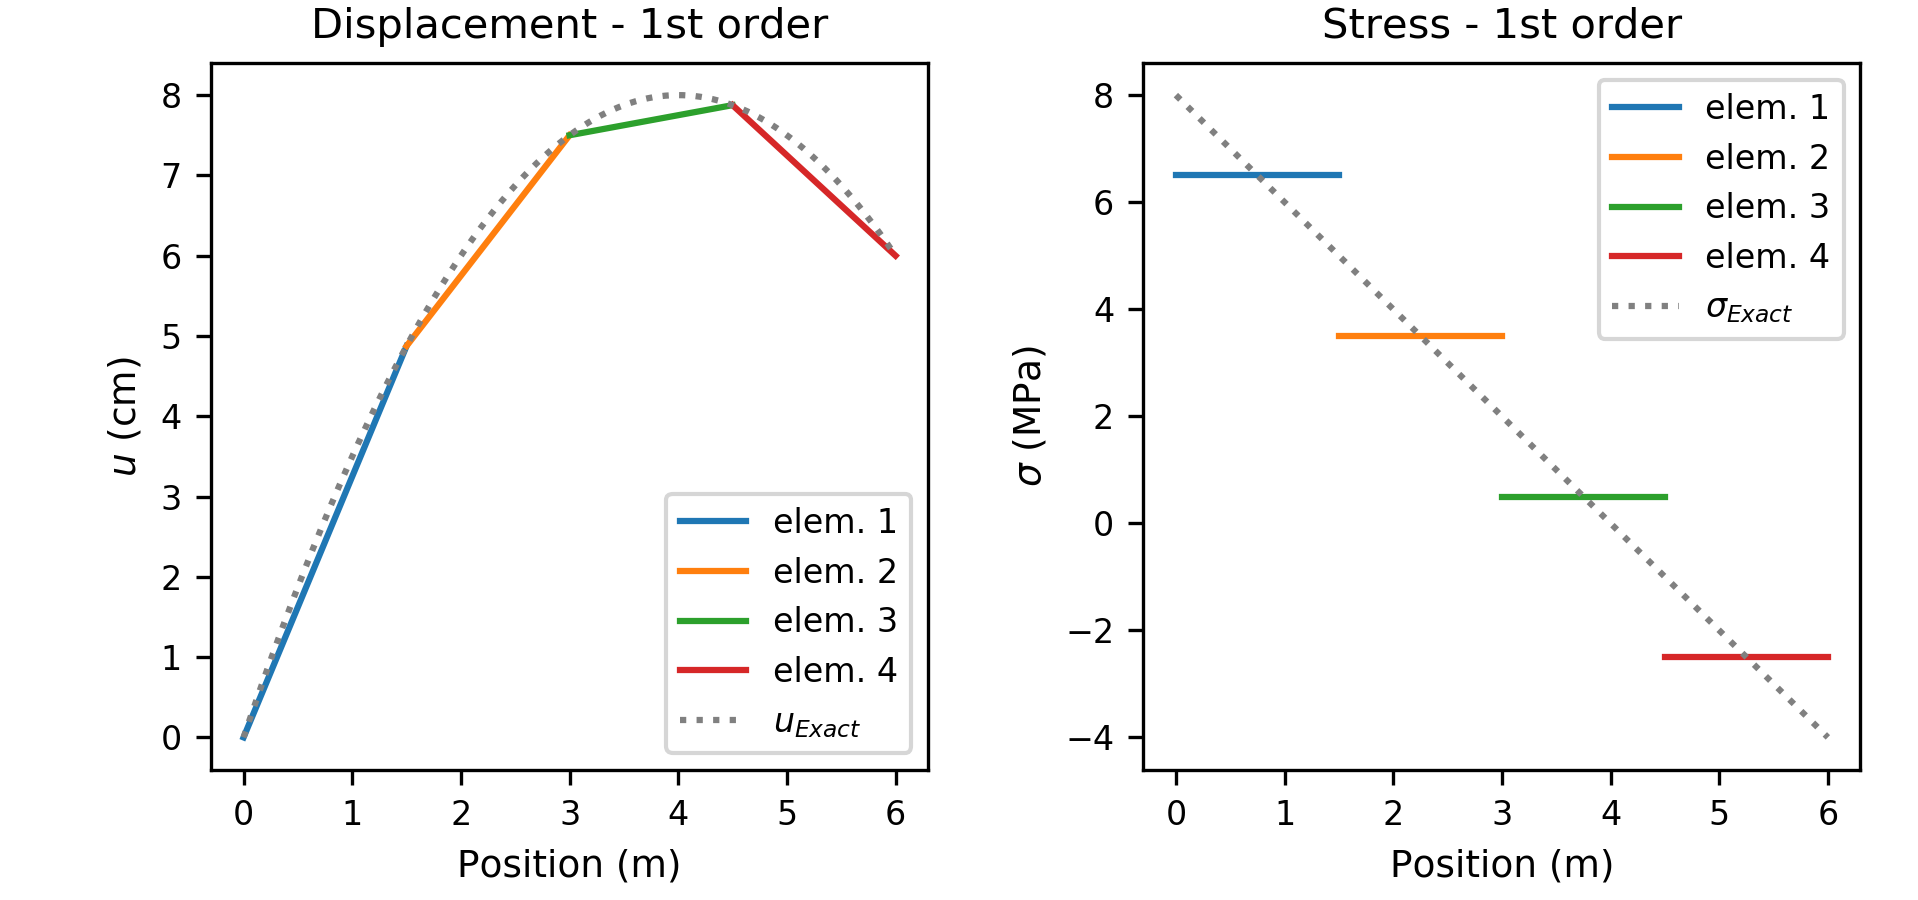
\includegraphics[width=0.9\linewidth]{1st_order_plot.png}
	\captionsetup{format=hang}
	\caption{Displacement and Stress calculated using linear shape functions compared to the exact solution.}
	\label{fig:1plot}
\end{figure}
\begin{figure}[h!]
	\centering
	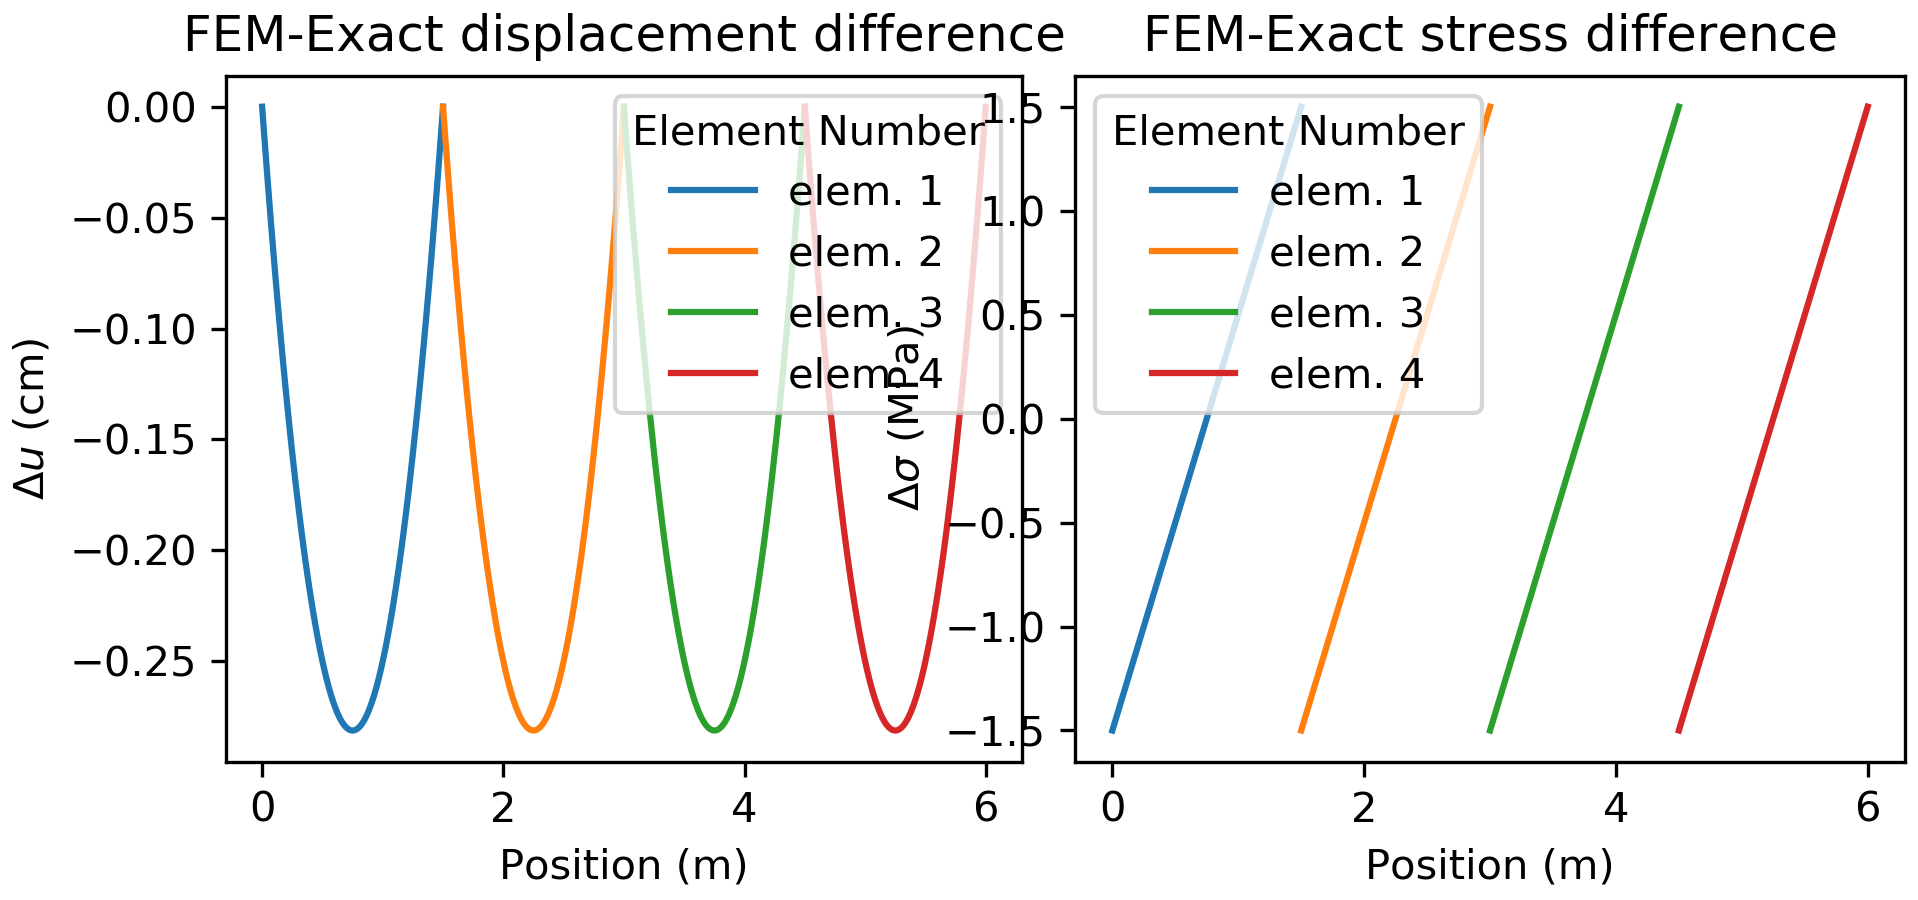
\includegraphics[width=0.9\linewidth]{1st_order_diffplot.png}
	\captionsetup{format=hang}
	\caption{Difference between the FEM and analytical displacement and stress using linear shape functions.}
	\label{fig:1diffplot}
\end{figure}
When using linear shape functions for the FEM model, we can see that there are huge differences to the exact solutions, particularly for the stress. If we were to repeat the calculations using more elements, one would expect the displacements to converge towards the analytical curve. We note that the FEM result for the displacements is exact at node points, and by increasing the number of nodes, we improve the result. In order for the stresses to do the same, the number of elements would have to be very large, but they would approach the exact curve eventually. In this case, the FEM result is exact in between the node points, and again, increasing the number of elements would improve the result, but since the deviation from the exact result is much greater away from these points, one would need many more elements to obtain an acceptable approximation of the exact values.
\newpage
\section{}
The elemental matrices and vectors for the quadratic shape function were found
by adapting the derivation provided for the linear shape function. The element
shape function matrices are given by
\begin{align}
    \bm{N^e} &= \frac{2}{(l^e)^e}
\end{align}

\begin{figure}[h!]
	\centering
	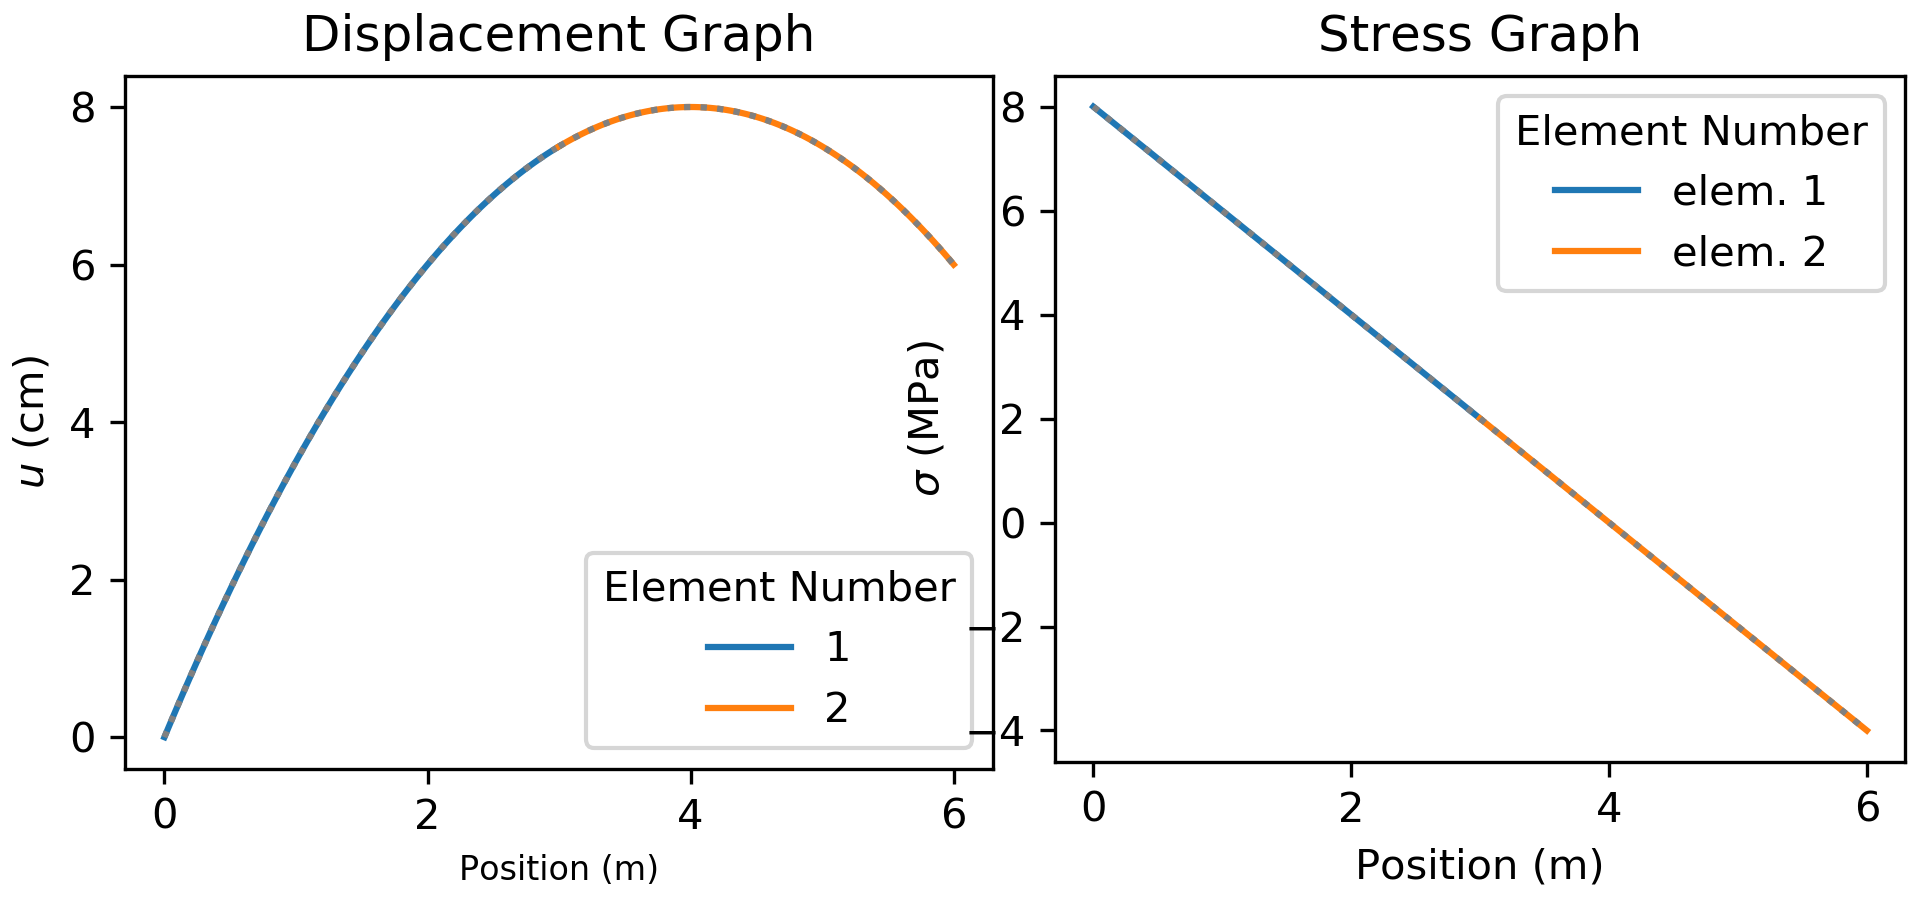
\includegraphics[width=0.9\linewidth]{2nd_order_plot.png}
	\captionsetup{format=hang}
	\caption{Displacement and Stress calculated using quadratic shape functions compared to the exact solution.}
	\label{fig:2plot}
\end{figure}
\begin{figure}[h!]
	\centering
	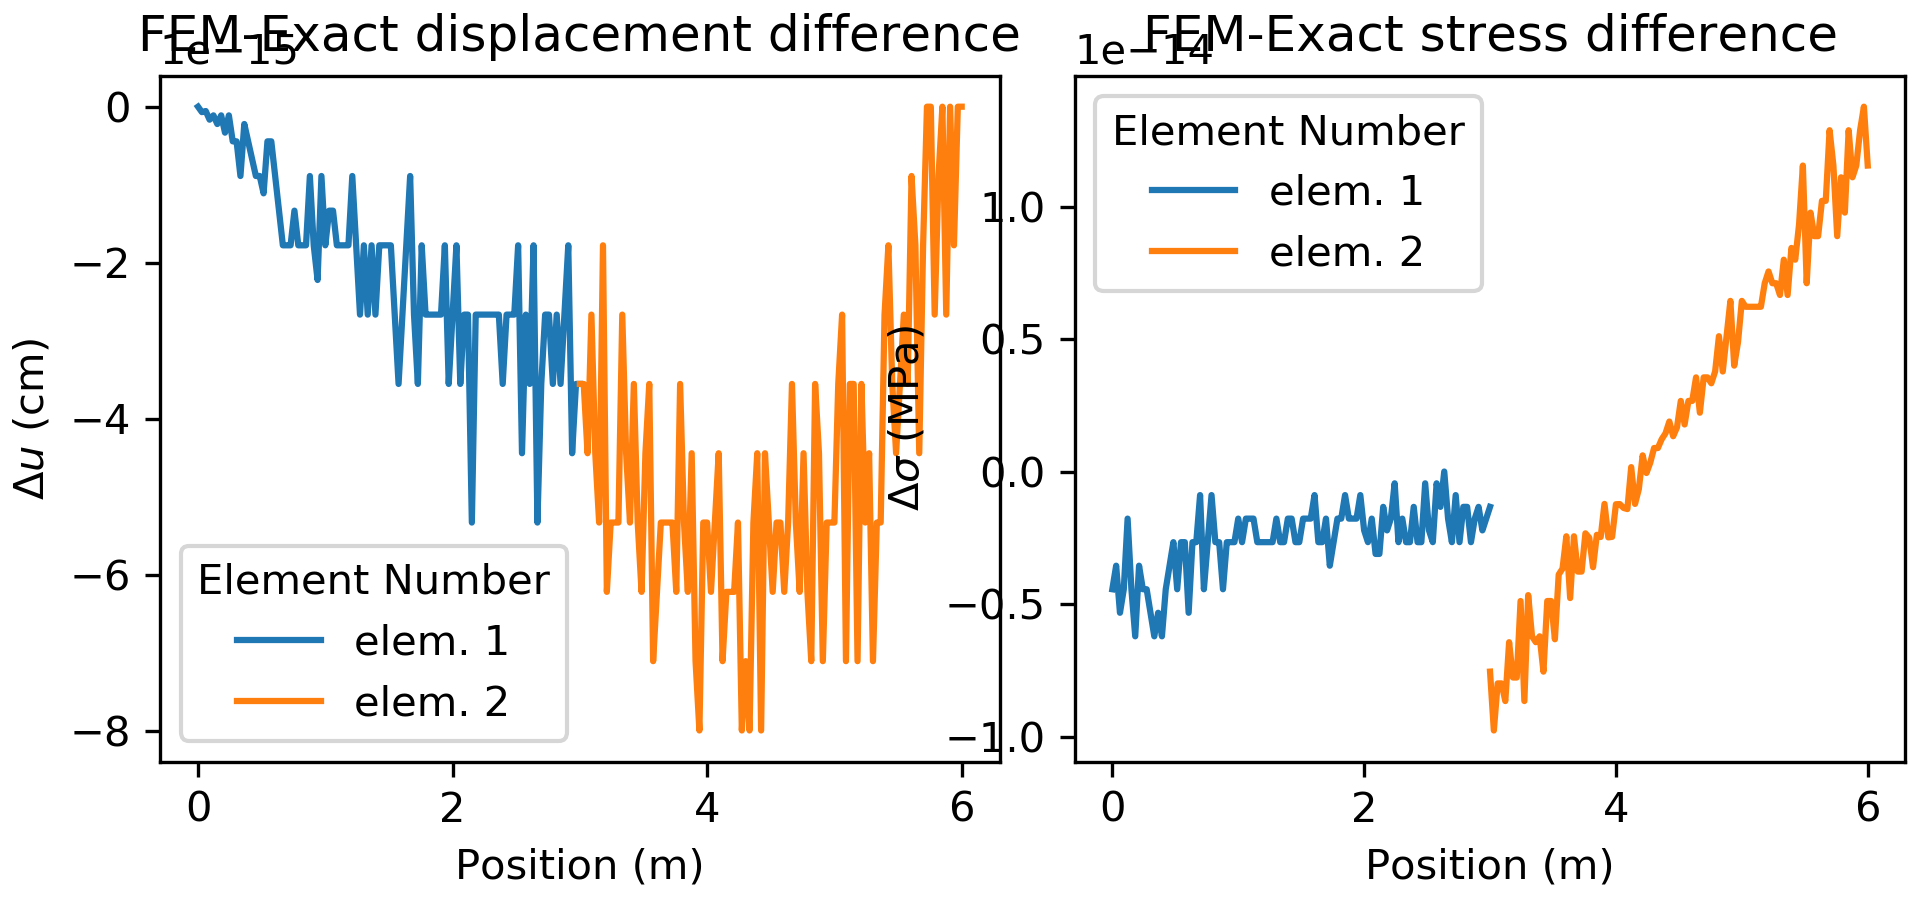
\includegraphics[width=0.9\linewidth]{2nd_order_diffplot.png}
	\captionsetup{format=hang}
	\caption{Difference between the FEM and analytical displacement and stress using quadratic shape functions.}
	\label{fig:2diffplot}
\end{figure}
For quadratic shape functions, we can see that the result is much better, even if only two elements are used. The differences between the analytical and the FEM result are so small (note the scale of the y-axis in figure \ref{fig:2diffplot}) that it seems impractical to employ higher-order shape functions - the result would likely not improve much. More precisely, this second-order FEM result is exact to the numerical precision of the IEEE 754 double-precision floating point standard used in most python environments.
\end{document}
